\documentclass{beamer}

% listings
\usepackage{listings}
\usepackage{xcolor}
\usepackage[]{sourcecodepro}	% Adobe Source Code Pro, included in texlive-fontsextra
\definecolor{light-gray}{gray}{0.96}
\definecolor{myblue}{rgb}{0,0,0.8}
\definecolor{mygreen}{rgb}{0,0.5,0}
\definecolor{mymauve}{rgb}{0.5,0,0.8}
\definecolor{mygray}{rgb}{0.5,0.5,0.5}
\lstset{
  language=C,
%  basicstyle=\small\sffamily,
  basicstyle=\small\ttfamily,
  keywordstyle=\color{myblue},
  commentstyle=\color{mygreen},
  stringstyle=\color{mymauve},
  numberstyle=\tiny\color{mygray},
  numbers=left,
  captionpos=b,
  abovecaptionskip=7pt,
  columns=flexible,
  showstringspaces=false,
  backgroundcolor=\color{light-gray},
  linewidth=\linewidth,		% Zeilenbreite
  breaklines=true,			% Zeileumbruch
  breakatwhitespace=false,	% Umbruch an Leerzeichen
  tabsize=2,
  keepspaces=true,
  extendedchars=true,
  xleftmargin=17pt,
  framexleftmargin=17pt,
%  frame=tb,
  frame=single,
  frameround=tttt,
}
\newcommand{\listingC}[2]
{
  \lstinputlisting[language=C,caption={#2},label=lst:#1]{../listings/18-file/#1}
}
\newcommand{\inlineC}[1]{\lstinline[language=C]$#1$}
\newcommand{\inlineML}[1]{\lstinline[language=ML]$#1$}
\newcommand{\inlineSh}[1]{\lstinline[language=Bash]$#1$}

%\usepackage[ampersand]{easylist}
\usepackage{skull}

% Tikz
\usepackage{tikz}
\usetikzlibrary{arrows, automata, positioning} % automata
%\tikzstyle{cfg}=[->,>=stealth',shorten >=1pt,auto,node distance=1.8cm,thick,every node/.style={rectangle,fill=gray!10,draw,font=\sffamily\bfseries}]
%\tikzstyle{cfgpath}=[every node/.style={font=\sffamily\small}]


% There are many different themes available for Beamer. A comprehensive
% list with examples is given here:
% http://deic.uab.es/~iblanes/beamer_gallery/index_by_theme.html
%\usetheme{AnnArbor}
%\usetheme{Antibes}
%\usetheme{Bergen}
%\usetheme{Berkeley}
%\usetheme{Berlin}
%\usetheme{Boadilla}
%\usetheme{boxes}
%\usetheme{CambridgeUS}
%\usetheme{Copenhagen}
%\usetheme{Darmstadt}
%\usetheme{default}
\usetheme{Frankfurt}
%\usetheme{Goettingen}
%\usetheme{Hannover}
%\usetheme{Ilmenau}
%\usetheme{JuanLesPins}
%\usetheme{Luebeck}
%\usetheme{Madrid}
%\usetheme{Malmoe}
%\usetheme{Marburg}
%\usetheme{Montpellier}
%\usetheme{PaloAlto}
%\usetheme{Pittsburgh}
%\usetheme{Rochester}
%\usetheme{Singapore}
%\usetheme{Szeged}
%\usetheme{Warsaw}

\title{Verifying Regular Safety Properties of C Programs Using the Static Analyzer Goblint}

% A subtitle is optional and this may be deleted
% \subtitle{Optional Subtitle}

\author{Ralf Vogler}
% - Give the names in the same order as the appear in the paper.
% - Use the \inst{?} command only if the authors have different
%   affiliation.

\institute[TUM] % (optional, but mostly needed)
{
  Department of Computer Science\\
  Technische Universit\"at M\"unchen}
% - Use the \inst command only if there are several affiliations.
% - Keep it simple, no one is interested in your street address.

\date{Master's thesis, 27.11.2013}
% - Either use conference name or its abbreviation.
% - Not really informative to the audience, more for people (including
%   yourself) who are reading the slides online

\subject{Theoretical Computer Science}
% This is only inserted into the PDF information catalog. Can be left
% out. 

% If you have a file called "university-logo-filename.xxx", where xxx
% is a graphic format that can be processed by latex or pdflatex,
% resp., then you can add a logo as follows:

% \pgfdeclareimage[height=0.5cm]{university-logo}{university-logo-filename}
% \logo{\pgfuseimage{university-logo}}

% Delete this, if you do not want the table of contents to pop up at
% the beginning of each subsection:
\AtBeginSubsection[]
{
  \begin{frame}<beamer>{Outline}
    \tableofcontents[currentsection,currentsubsection]
  \end{frame}
}

% Let's get started
\begin{document}

\begin{frame}
  \titlepage
\end{frame}

\begin{frame}{Outline}
  \tableofcontents
  % You might wish to add the option [pausesections]
\end{frame}

% Section and subsections will appear in the presentation overview
% and table of contents.

\section{Motivation}

\begin{frame}{Motivation}
\begin{itemize}
\item Static typing the C way:
	\begin{itemize}
	\item pointers for everything
	\item NULL on error
	\end{itemize}
\item Types do not enforce correct API usage
	\begin{itemize}
	\item Misuse can easily happen
	\item Program compiles, but fails at run-time
		\begin{itemize}
		\item segfault
		\item leaks
		\item memory corruption
		\item unintended behavior \ldots
		\end{itemize}
	\end{itemize}
	\item Hard to debug
\end{itemize}
\end{frame}


\section{Verifying correct usage of file handles}

\subsection{Common problems}

\begin{frame}{The ordinary life of a file handle}
\begin{itemize}
\item How file handles should be used:
%	\begin{itemize}
%	\item uninitialized
%	\item opened in mode x / failed to open
%	\item read and/or write
%	\item closed
%	\end{itemize}
\end{itemize}
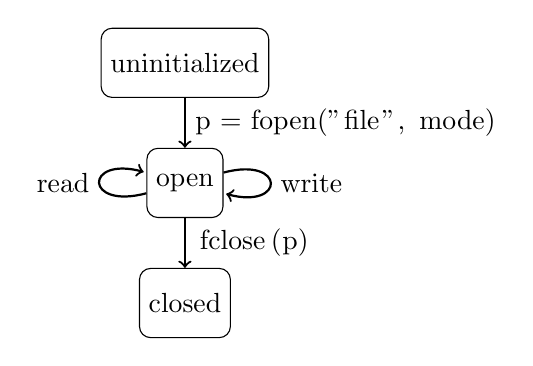
\begin{tikzpicture}[every state/.style={draw,rectangle, rounded corners},node distance=1.8em]
  \node[state] (A) {uninitialized};
  \node[state] (B) [below= of A] {open};
  \node[state] (C) [below= of B] {closed};

  \path[thick,-to]
    (A) edge node[right] {\inlineC{p = fopen("file", mode)}} (B)
    (B) edge [loop left] node[left] {read} (B)
    (B) edge [loop right] node[right] {write} (B)
    (B) edge node[right] {\inlineC{fclose(p)}} (C)
  ;
\end{tikzpicture}
%\begin{tikzpicture}[style=cfg]
%  \node (1) {uninitialized};
%  \node [below of=1] (2) {opened};
%  \node [below of=2] (3) {closed};
%
%  \path[style=cfgpath]
%    (1) edge node {fopen} (2)
%    (2) edge [loop right] node {fprintf} (2)
%    (2) edge node {fscanf} (2)
%    (2) edge node {fclose()} (3)
%  ;
%\end{tikzpicture}
\begin{itemize}
\item Any deviation from this pattern probably is an error
\end{itemize}
\end{frame}

\begin{frame}[fragile]{Opening files}
\begin{lstlisting}
#include <stdio.h>

int main(){
    FILE *fp;
    fp = fopen("log.txt", "a");
    fprintf(fp, "Testing...\n"); // log something
    fclose(fp);
    // do important things
}
\end{lstlisting}
\begin{itemize}
\item Appends text to file (creates file if it does not exist)
\item Everything ok?
\pause
\item $\skull$ segfault if file exists but no write-access!
\end{itemize}
\end{frame}

\begin{frame}[fragile]{Opening files}{The right way}
\begin{lstlisting}
#include <stdio.h>
#include <stdlib.h>

int main(){
    FILE *fp;
    fp = fopen("log.txt", "a");
    if(fp){
        printf("file opened");
        fprintf(fp, "Testing...\n");
        fclose(fp);
    }else{
        perror("failed to open file");
        // handle error
        return EXIT_FAILURE;
    }
    return EXIT_SUCCESS;
}
\end{lstlisting}
\end{frame}

\begin{frame}[fragile]{Not opening files}
\begin{lstlisting}
#include <stdio.h>

FILE *fp;

int main(){
    fprintf(fp, "Testing...\n"); // WARN: writing to unopened file handle fp
    fclose(fp); // WARN: closeing unopened file handle fp
}
\end{lstlisting}
\begin{itemize}
\item Dereferencing an uninitialized pointer is undefined behavior!
	\begin{itemize}
	\item Usually leads to segfault, but might do anything
	\item May result in optimization-unstable code
	\end{itemize}
\end{itemize}
\end{frame}

%\begin{frame}[fragile]{Not opening files}{Optimization-unstable code}
%\begin{lstlisting}
%#include <stdio.h>
%
%int main(){
%    struct *foo = ...;
%    FILE *fp;
%    fp = foo->fp; // undefined if foo was NULL
%    if(!foo) // optimized away
%    	fp = fopen("log.txt", "a");
%    fprintf(fp, "Testing...\n"); // WARN: MAYBE writing to unopened file handle fp
%    fclose(fp); // WARN: MAYBE closeing unopened file handle fp
%}
%\end{lstlisting}
%\begin{itemize}
%\item Works with \verb|-O0|
%\end{itemize}
%\end{frame}

\begin{frame}[fragile]{Closing files}
\begin{lstlisting}
#include <stdio.h>

int main(){
    char text[20];
    FILE *fp;
    fp = fopen("test.txt", "w"); // WARN: file is never closed
    fprintf(fp, "Shared content");
    // fclose();
    printf("enter some text: ");
    // file stays empty until exit
    fgets(text, sizeof text, stdin);
    printf("text = \"%s\"\n", text);
} // WARN: unclosed files: fp
\end{lstlisting}
\begin{itemize}
\item Not closing files is bad practice!
	\begin{itemize}
	\item Flushing
	\item System limit on open file handles
	\end{itemize}
\end{itemize}
\end{frame}

\begin{frame}[fragile]{Wrong open mode}
\begin{itemize}
\item Writing to read-only file:
\end{itemize}
\begin{lstlisting}
#include <stdio.h>

int main(){
    FILE *fp;
    fp = fopen("test.txt", "r"); 
    fprintf(fp, "Testing...\n"); // WARN: writing to read-only file handle fp
    fclose(fp);
}
\end{lstlisting}
\begin{itemize}
\item Hard to find bugs:
	\begin{itemize}
	\item Writing to read-only: writes nothing
	\item Reading from write-only: behaves like empty file
	\end{itemize}
\end{itemize}
\end{frame}

\subsection{Implementation}

\begin{frame}[fragile]{Domain}
\begin{itemize}
\item Map from L-Values to domain for file handle:
\end{itemize}
\begin{lstlisting}[language=ML]
type loc = location list
type mode = Read | Write
type state = Open of string*mode | Closed | Error
type record = { key: Lval.CilLval.t; loc: loc; state: state }
type t = record Set.t * record Set.t (* must, may *)
\end{lstlisting}
\begin{itemize}
\item Location and filename are not needed for determining correct state
\end{itemize}
\end{frame}

\begin{frame}[fragile]{Location of warnings}
\begin{lstlisting}
#include <stdio.h>

FILE* myfopen(char* filename){
    FILE *fp;
    fp = fopen(filename, "a");
    if(fp == NULL) exit(1);
    return fp;
}

int main(){
    FILE *fp1; FILE *fp2;
    fp1 = myfopen("test1.txt");
    fp2 = myfopen("test2.txt"); // WARN: file is never closed
    fclose(fp1);
    // fclose(fp2);
} // WARN: unclosed files: fp2
\end{lstlisting}
\end{frame}

\begin{frame}[fragile, squeeze]{Location of warnings}{Avoid infinite strictly ascending chains!}
\begin{lstlisting}
#include <stdio.h>

FILE* myfopen(char* filename){
    int b;
    if(b)
        return myfopen(filename);
    else
        return fopen(filename, "a");
}

int main(){
    FILE *fp; fp = myfopen("test.txt");
    fprintf(fp, "Testing...\n");
    fclose(fp);
}
\end{lstlisting}
\begin{itemize}
\item Program terminates pretty fast but analysis would not!
\end{itemize}
\end{frame}


\section{A specification language}

\subsection{Implementation}

\begin{frame}[fragile]{Implementation}
\begin{itemize}
\item Domain similar to file handles:
\end{itemize}
\begin{lstlisting}[language=ML]
type state = string
type record = {key: Lval.CilLval.t; loc: location list; state: state}
type t = record Set.t * record Set.t (* must, may *)
\end{lstlisting}
\begin{itemize}
\item Use a Mealy machine $(S, s_0, \Sigma, \Lambda, T, G)$ to determine the output by the current state and input
\item States, transitions and warnings are defined in a specification file
\end{itemize}
\end{frame}

\subsection{Format}

\begin{frame}[fragile]{Format}
\begin{itemize}
\item Outputs $\Lambda$
\item Transitions $T' : S \times \Sigma \to S \times \Lambda$
\end{itemize}
\begin{lstlisting}
// warnings
w1  "file handle is not saved"
w2  "closeing unopened file handle"

// transitions
a   -w1>    a   fopen(_)
a   -w2>    a   fclose($fp)
a   ->      b   $fp = fopen(_)
...
\end{lstlisting}
\begin{itemize}
\item Start state of first transition is $s_0$
\item Key for map is denoted by \inlineC{\$}
\item Pattern matching
\end{itemize}
\end{frame}


\section{Example use cases}

\subsection{File handles redux}

\begin{frame}[fragile]{File handles redux}
\begin{lstlisting}[basicstyle=\tiny\ttfamily,]
w1 "file handle is not saved!"
w2 "closeing unopened file handle $"
w3 "writing to unopened file handle $"
w4 "writing to read-only file handle $"
w5 "closeing already closed file handle $"
w6 "writing to closed file handle $"
w7 "overwriting still opened file handle $"
w8 "unrecognized file open mode for file handle $"

1          -w1> 1           fopen(_)
1          -w2> 1           fclose($fp)
1          -w3> 1           fprintf($fp, _)
1          ->   open_read   $fp = fopen(_, "r")
1          ->   open_write  $fp = fopen(_, r"[wa]") // regex, see OCaml doc
1          -w8> 1           $fp = fopen(_, _)

open_read  -w4>  open_read  fprintf($fp, _)
open_read  -w7>> 1          $fp = fopen(_, _)
open_write -w7>> 1          $fp = fopen(_, _)

open_read  -> closed        fclose($fp)
open_write -> closed        fclose($fp)

closed     -w5> closed      fclose($fp)
closed     -w6> closed      fprintf($fp, _)
closed     ->>  1           _ // let state 1 handle the rest
// setup which states are end states
end: 1, closed
// warning for all entries that are not in an end state
!end "file is never closed"
!end@return "unclosed files: $"
\end{lstlisting}
\end{frame}

\begin{frame}[fragile]{File handles redux}{Realistic fopen}
\begin{itemize}
\item Caveat: specification is optimistic about opening files
\item \inlineC{fopen()} might fail:
\end{itemize}
\begin{lstlisting}[basicstyle=\scriptsize\ttfamily]
...
// go to unchecked states first
1           -> u_open_read  $fp = fopen(_, "r")
1           -> u_open_write $fp = fopen(_, r"[wa]") // regex, see OCaml doc
1           -w8> 1          $fp = fopen(_, _)

// define possible branches
u_open_read  -> 1           branch($fp==0, true)
u_open_read  -> open_read   branch($fp==0, false)
u_open_write -> 1           branch($fp==0, true)
u_open_write -> open_write  branch($fp==0, false)
...
\end{lstlisting}
\end{frame}

\subsection{Dynamic memory allocation}

\begin{frame}[fragile]{Dynamic memory allocation}{Example}
\begin{itemize}
\item Correct usage: 1. \inlineC{malloc}, 2. use memory, 3. \inlineC{free}
\end{itemize}
\begin{lstlisting}[basicstyle=\scriptsize\ttfamily]
#include <stdlib.h>
#include <stdio.h>

int main(){
  int *ip;
  //*ip = 5; // write: segfault
  //printf("%i", *ip); // read: segfault
  ip = malloc(sizeof(int)); // allocate memory
  if(ip == NULL) return 1; // success check

  *ip = 5; // work with memory

  free(ip); // free memory
  //free(ip); // crash: double free or corruption
  *ip = 5; // undefined but no crash
  printf("%i", *ip); // undefined but prints 5
  ip = NULL; // make sure the pointer is not used anymore
  //*ip = 5; // segfault
}
\end{lstlisting}
\end{frame}

\begin{frame}[fragile, shrink]{Dynamic memory allocation}{Specification}
\begin{lstlisting}[basicstyle=\scriptsize\ttfamily]
w1 "pointer is not saved [leak]"
w2 "freeing unallocated pointer $ [segfault?]"
w3 "writing to unallocated pointer $ [segfault?]"
w4 "overwriting unfreed pointer $ [leak]"
w4 "freeing already freed pointer $ [double free!]"

1        -w1> 1        malloc(_)
1        -w2> 1        free($p)
1        -w3> 1        *$p = _
1        ->   u_alloc  $p = malloc(_)

u_alloc  ->   1        branch($p==0, true)
u_alloc  ->   alloc    branch($p==0, false)

alloc    -w4> alloc    $p = malloc(_)
alloc    ->   freed    free($p)

freed    -w5> freed    free($p)
freed    ->>  1        _ // let state 1 handle the rest
// setup which states are end states
end: 1, freed
// warning for all entries that are not in an end state
!end "pointer is never freed"
!end@return "unfreed pointers: $"
\end{lstlisting}
\end{frame}


\section{Demo}

\begin{frame}[fragile]{Demo}
\begin{center}
%{\Huge Demo}
%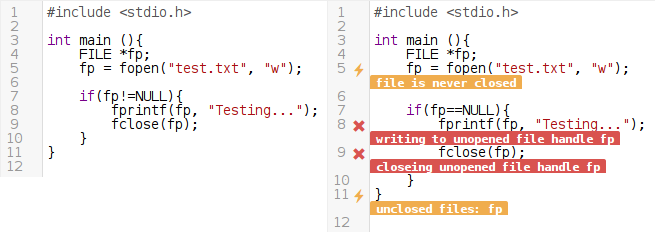
\includegraphics[width=\linewidth]{graphics/webapp-26-27.png}
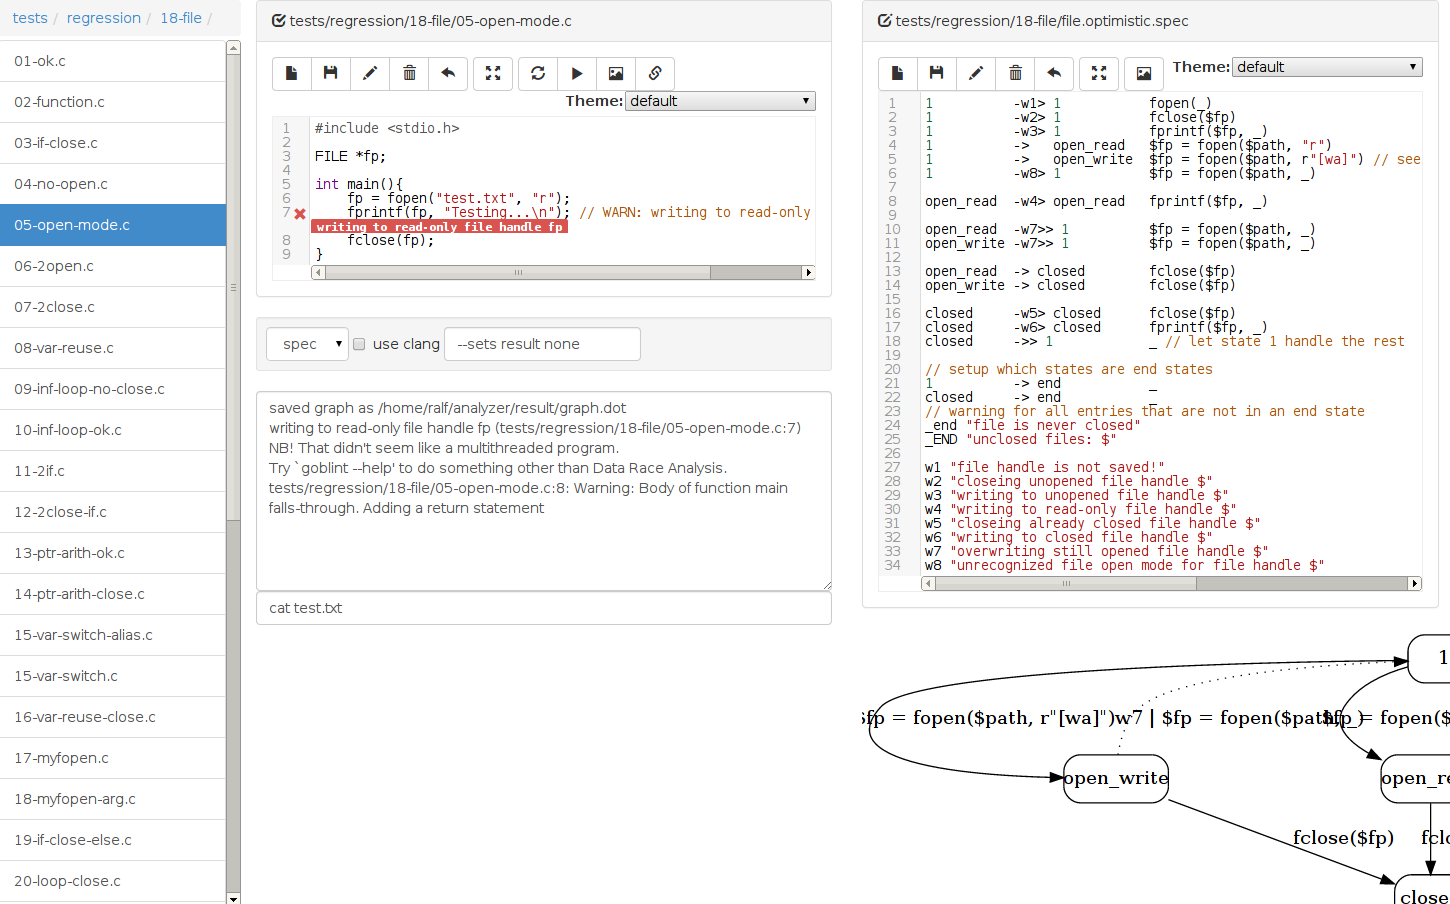
\includegraphics[width=\linewidth]{graphics/webapp_small.png}
\end{center}

\end{frame}



%\begin{frame}{Blocks}
%\begin{block}{Block Title}
%You can also highlight sections of your presentation in a block, with it's own title
%\end{block}
%\begin{theorem}
%There are separate environments for theorems, examples, definitions and proofs.
%\end{theorem}
%\begin{example}
%Here is an example of an example block.
%\end{example}
%\end{frame}

%% Placing a * after \section means it will not show in the
%% outline or table of contents.
%\section*{Summary}
%
%\begin{frame}{Summary}
%  \begin{itemize}
%  \item
%    The \alert{first main message} of your talk in one or two lines.
%  \item
%    The \alert{second main message} of your talk in one or two lines.
%  \item
%    Perhaps a \alert{third message}, but not more than that.
%  \end{itemize}
%  
%  \begin{itemize}
%  \item
%    Outlook
%    \begin{itemize}
%    \item
%      Something you haven't solved.
%    \item
%      Something else you haven't solved.
%    \end{itemize}
%  \end{itemize}
%\end{frame}
%
%
%
%% All of the following is optional and typically not needed. 
%\appendix
%\section<presentation>*{\appendixname}
%\subsection<presentation>*{For Further Reading}
%
%\begin{frame}[allowframebreaks]
%  \frametitle<presentation>{For Further Reading}
%    
%  \begin{thebibliography}{10}
%    
%  \beamertemplatebookbibitems
%  % Start with overview books.
%
%  \bibitem{Author1990}
%    A.~Author.
%    \newblock {\em Handbook of Everything}.
%    \newblock Some Press, 1990.
% 
%    
%  \beamertemplatearticlebibitems
%  % Followed by interesting articles. Keep the list short. 
%
%  \bibitem{Someone2000}
%    S.~Someone.
%    \newblock On this and that.
%    \newblock {\em Journal of This and That}, 2(1):50--100,
%    2000.
%  \end{thebibliography}
%\end{frame}

\end{document}
